\section{Introduction}
Most health performance indicators are built from records that start with a clinical encounter: claims, discharge abstracts, registries and notifiable-disease reports. A person whose diabetes or hypertension has never been detected does not appear in any of them. The US National Health and Nutrition Examination Survey (NHANES) is different because it interviews a national probability sample at home and then measures the same people in a mobile examination centre (MEC). It can therefore count disease that the health system has not yet seen. National estimates put the undiagnosed share of US diabetes between one fifth and one quarter \cite{wang2021,fang2022,gwira2024}.

This project had two aims: to turn NHANES 2017--2018 into a three-tier key performance indicator (KPI) dashboard in which every number is a design-based estimate with a valid interval, and to test whether non-laboratory information is enough to find people with undiagnosed diabetes. The contributions are (i) a reproducible pipeline producing 612 survey-weighted estimates with Taylor-linearised errors, $t$-based intervals and NCHS suppression; (ii) an income concentration analysis with a tie correction, pooled and within age bands; (iii) a nested, survey-weighted comparison of four machine-learning (ML) models with an adapted American Diabetes Association (ADA) risk score and seven published benchmarks; and (iv) a Streamlit dashboard that only reads the audited estimates.

\section{Related Work}
\subsubsection*{Undiagnosed diabetes and hypertension in NHANES} Wang \textit{et al.} found that 23.3\% of US diabetes was undiagnosed in 2017--2018 \cite{wang2021}. Fang \textit{et al.} showed that this share depends on whether a confirmatory second test is required \cite{fang2022}, and studied control trends and screening eligibility \cite{fang2021}; later work extends the series to 2021--2023 \cite{gwira2024,cdc_ndsr}. For blood pressure, control declined after 2013--2014 \cite{muntner2020,muntner2022}, and later cycles report awareness and control \cite{ostchega2020,fryar2024}. Hales \textit{et al.} give the reference obesity estimate \cite{hales2020}.

\subsubsection*{Machine learning for undiagnosed diabetes} De Silva \textit{et al.} found that logistic regression (LR), random forest (RF) and neural networks did not significantly beat the ADA risk test \cite{bang2009} for undiagnosed diabetes in NHANES \cite{desilva2021}; Choi \textit{et al.} found tree ensembles ahead of Korean risk scores \cite{choi2023}. Other NHANES studies report AUCs from 0.75 to 0.91 for outcomes from fasting-glucose to self-reported diabetes \cite{qin2022,riverosperez2025,liu2025,yang2026,yoo2026}, but none of the full texts we checked used the survey weights, which change both the fitted model and its estimated performance \cite{macnell2023,kim2026}.

\subsubsection*{Inequality measurement and dashboards} The concentration index measures how a health variable is distributed across income ranks; Erreygers corrected it for bounded outcomes \cite{erreygers2009}, and recent work applies it along the care cascade \cite{vu2026,okova2026}. Dashboard reviews call for actionable indicators with stated uncertainty \cite{ivankovic2021,schulze2023}. Public NHANES has no geography, so maps need model-based products such as CDC PLACES \cite{greenlund2022}.

\section{Data and Methodology}
\begin{figure*}[t]
\centering
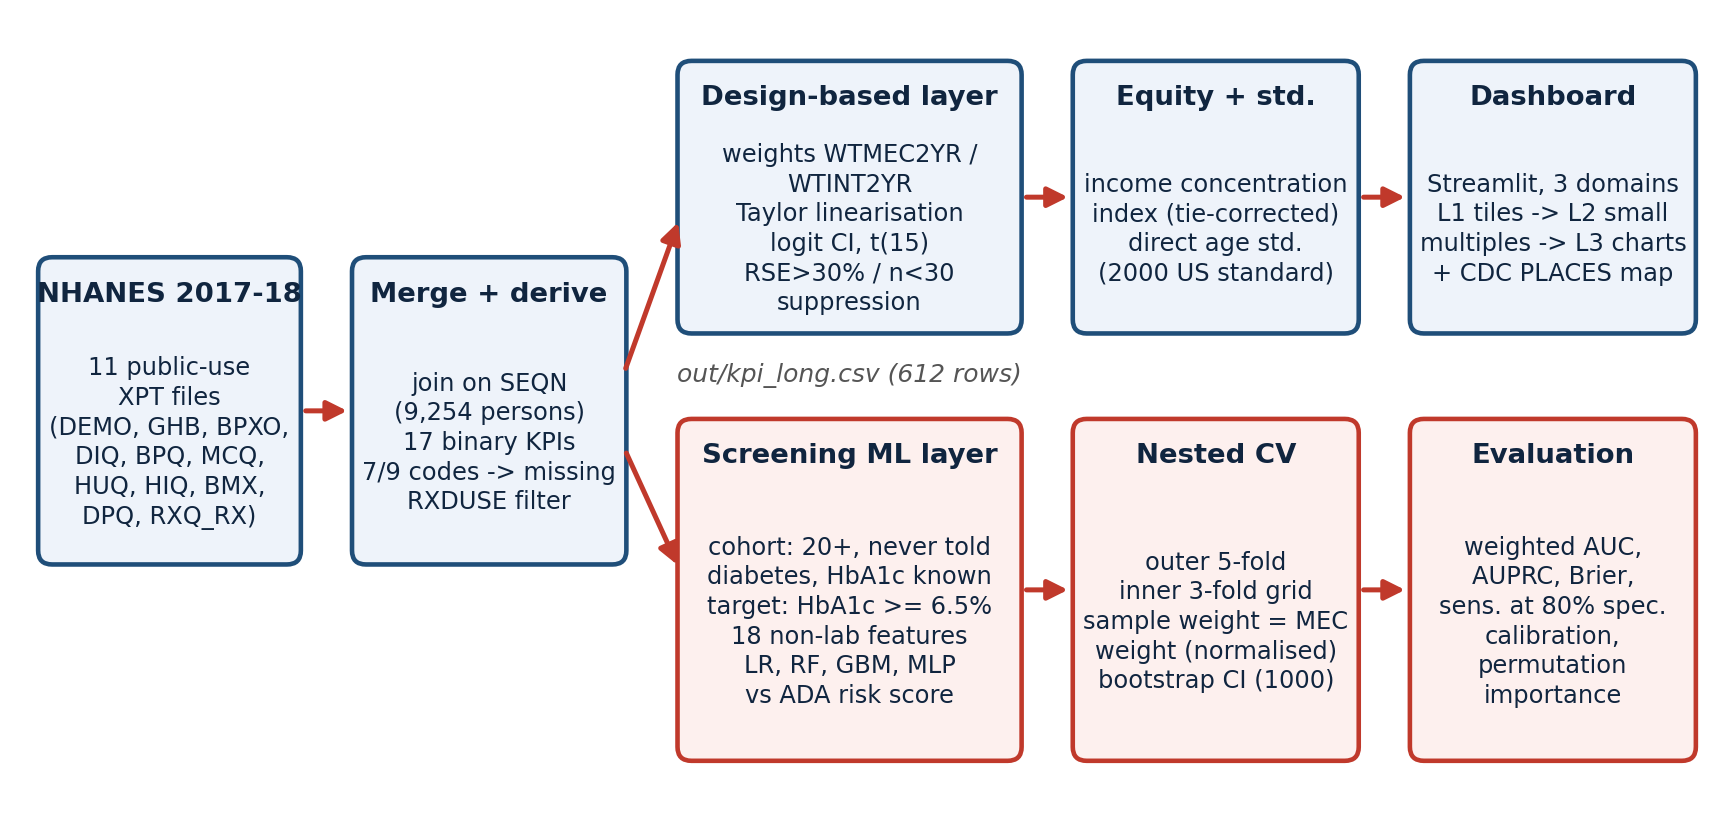
\includegraphics[width=0.66\textwidth]{figures/architecture.png}
\caption{System architecture. The upper path produces the design-based KPI estimates read by the dashboard; the lower path trains and evaluates the screening models on the same analytic file.}
\label{fig:arch}
\end{figure*}
\subsection{Data}
We used 11 public-use NHANES 2017--2018 files: demographics (DEMO), glycohaemoglobin (GHB), oscillometric blood pressure (BPXO), body measures (BMX), the diabetes (DIQ), blood-pressure (BPQ), medical-conditions (MCQ), utilisation (HUQ), insurance (HIQ) and PHQ-9 depression (DPQ) questionnaires, and prescription medicines (RXQ\_RX). Files were merged on the respondent identifier SEQN, giving 9,254 persons with no duplicates. Codes 7 and 9 (refused, don't know) were set to missing, and prescription counts used only rows with \texttt{RXDUSE}$=1$.

\subsection{Indicators}
Seventeen binary indicators were defined for adults aged 18 and over, grouped into three domains. \textit{Utilisation and patient experience}: fair or poor self-rated health, overnight admission in the past 12 months, four or more care contacts, having a usual source of care, and the emergency department as usual source. \textit{Chronic disease}: HbA1c $\geq$6.5\% (laboratory diabetes), self-reported diagnosis, any diabetes, undiagnosed diabetes (laboratory-positive and never told, among the laboratory-positive), prediabetes (HbA1c 5.7--6.4\%), measured hypertension at 130/80 and 140/90 mmHg (mean of up to three readings), undiagnosed hypertension at each threshold, obesity (BMI $\geq$30) and depression (PHQ-9 $\geq$10). \textit{Access}: uninsured and polypharmacy ($\geq$5 prescriptions). Respondents who answered ``borderline'' to the diabetes question were treated as diagnosed in the primary analysis and as undiagnosed in a sensitivity analysis.

\subsection{Design-based estimation}
NHANES is a stratified, multistage cluster sample, so estimates use the MEC weight $w_i$ (\texttt{WTMEC2YR}) for examination or laboratory indicators and the interview weight (\texttt{WTINT2YR}) otherwise. A prevalence is the ratio estimator
\begin{equation}
\hat p = \frac{\sum_i w_i y_i}{\sum_i w_i},
\end{equation}
and its variance is obtained by Taylor linearisation with a with-replacement approximation over strata $h$ and primary sampling units (PSUs) $j$:
\begin{equation}
\widehat{\mathrm{Var}}(\hat p) = \frac{1}{\left(\sum_i w_i\right)^2}\sum_{h}\frac{n_h}{n_h-1}\sum_{j=1}^{n_h}\left(z_{hj}-\bar z_h\right)^2,
\end{equation}
where $z_{hj}=\sum_{i\in(h,j)} w_i (y_i-\hat p)$ and $n_h$ is the number of PSUs in stratum $h$. The design has 30 PSUs in 15 strata, so the degrees of freedom are $d=30-15=15$ and intervals use $t_{0.975,15}=2.131$ instead of 1.96. Intervals are built on the logit scale so that they stay inside $[0,1]$:
\begin{equation}
\mathrm{logit}^{-1}\!\left(\mathrm{logit}(\hat p)\pm t_{0.975,d}\,\frac{\widehat{\mathrm{SE}}(\hat p)}{\hat p(1-\hat p)}\right).
\end{equation}
Following the NCHS presentation standard, a cell is suppressed when its relative standard error $\mathrm{RSE}=100\,\widehat{\mathrm{SE}}/\hat p$ exceeds 30\% or its unweighted $n$ is below 30. Rates are reported per 100,000 adults ($10^5\hat p$). Each indicator is estimated overall and by age band, sex, age by sex, race and ethnicity, income-to-poverty-ratio (PIR) quintile and number of chronic conditions, giving 612 cells.

\subsection{Income concentration index}
Respondents are ranked by PIR. The weighted fractional rank of person $i$ is $R_i$; because PIR is top-coded at 5.0, all tied values receive the midpoint of their block of cumulative weight. The relative concentration index is
\begin{equation}
C = \frac{2}{\mu}\,\mathrm{cov}_w\!\left(y_i, R_i\right),
\end{equation}
where $\mu$ is the weighted mean of $y$. $C<0$ means the condition is concentrated among poorer adults. For a binary outcome, the Erreygers corrected index is $E=4\mu C$ \cite{erreygers2009}; we report both. Indices are computed for adults only and also within 10-year age bands, because disease prevalence rises with age while low-PIR adults are younger on average.

\subsection{Direct age standardisation}
Age-standardised prevalences use the year-2000 US standard population in eight adult groups,
\begin{equation}
\hat p_{\mathrm{std}} = \frac{\sum_g s_g\,\hat p_g}{\sum_g s_g},\qquad
\widehat{\mathrm{Var}}(\hat p_{\mathrm{std}}) = \frac{\sum_g s_g^2\,\widehat{\mathrm{Var}}(\hat p_g)}{\left(\sum_g s_g\right)^2},
\end{equation}
where $s_g$ is the standard weight of group $g$. The 15--24 standard weight was split as 7/10 to approximate the 18--24 group, and suppressed age groups were dropped with renormalisation.

\subsection{Dashboard}
Level~1 tiles show each headline rate with its interval, RSE and $n$; a tile filters the Level~2 small multiples (age, sex, race and ethnicity, PIR quintile); Level~3 holds analytical charts (multimorbidity heatmap, population pyramid, Healthy People 2030 bar-in-bar, access by income, burden treemap). Suppressed cells appear as grey placeholders, never as zeros. A separate page maps CDC PLACES county estimates aggregated to states with population weights, labelled as a model-based source.

\subsection{Screening model}
\textit{Cohort and target.} Adults aged 20+ who said they had never been told they had diabetes and had an HbA1c result; the target was HbA1c $\geq$6.5\%.

\textit{Features.} Eighteen non-laboratory inputs: age, sex, race and ethnicity, PIR, education, BMI, waist circumference, waist-to-height ratio, mean systolic and diastolic pressure, told high blood pressure, told high cholesterol, family history of diabetes, self-rated health, PHQ-9 score, number of prescriptions, insurance and usual source of care. Missing numeric values were imputed with the training-fold median plus a missingness indicator.

\textit{Models.} Let $\mathbf{x}_i$ be the feature vector and $\tilde w_i=w_i/\bar w$ the normalised MEC weight. Logistic regression models $P(y_i=1\mid\mathbf{x}_i)=\sigma(\beta_0+\boldsymbol\beta^\top\mathbf{x}_i)$ and minimises the weighted, class-balanced penalised log-loss
\begin{equation}
\mathcal{L}(\boldsymbol\beta)=-\sum_i \tilde w_i\,c_{y_i}\!\left[y_i\log\hat\pi_i+(1-y_i)\log(1-\hat\pi_i)\right]+\frac{\lVert\boldsymbol\beta\rVert_2^2}{2C_{\mathrm{reg}}},
\end{equation}
where $c_{y}$ is the inverse class frequency. The random forest averages $B=500$ trees grown on bootstrap samples with weighted Gini splits. Histogram gradient boosting builds an additive model $F_M(\mathbf{x})=\sum_{m=1}^{M}\eta f_m(\mathbf{x})$, where each tree $f_m$ is fitted to the gradient of the weighted log-loss with step size $\eta$ and an $L_2$ leaf penalty $\lambda$. The multilayer perceptron (MLP) has one or two ReLU layers trained with Adam and early stopping; it cannot take sample weights, so it is the only unweighted learner. The baseline is the ADA risk test \cite{bang2009}: age (0--3 points), male sex (1), family history (1), hypertension (1) and BMI (0--3). Gestational diabetes and physical activity were not in the downloaded files, so the adapted score has a maximum of 9 instead of 11; the usual high-risk cut-off is $\geq$5.

\textit{Validation.} Performance was estimated with nested stratified cross-validation: five outer folds for testing and, inside each training fold, a three-fold grid search that selects hyperparameters by weighted AUC. The weighted AUC is
\begin{equation}
\mathrm{AUC}_w=\frac{\sum_{i:y_i=1}\sum_{k:y_k=0}\tilde w_i\tilde w_k\,\mathbb{1}[\hat s_i>\hat s_k]}{\sum_{i:y_i=1}\tilde w_i\;\sum_{k:y_k=0}\tilde w_k},
\end{equation}
with ties counted as one half. We also report the weighted area under the precision--recall curve (AUPRC), weighted Brier score and sensitivity at 80\% specificity. A 95\% interval for the pooled out-of-fold AUC, and for each model's AUC difference from the ADA score, came from 1,000 bootstrap resamples. Permutation importance (drop in weighted AUC, 10 repeats) was computed for the best model.

\subsection{Testing environment and hyperparameters}
All analysis ran in Python 3.12 (pandas 3.0, NumPy 2.0, SciPy 1.17, scikit-learn 1.8) on a Windows 11 laptop, with random seed 42 for every split and learner. Table~\ref{tab:hp} lists the analytic settings and search grids.

\begin{table}[t]
\caption{Analytic Settings and Hyperparameter Search Space}
\label{tab:hp}
\centering
\footnotesize
\setlength{\tabcolsep}{3pt}
\begin{tabular}{@{}p{2.3cm}p{5.6cm}@{}}
\toprule
\textbf{Component} & \textbf{Setting} \\
\midrule
Survey design & strata \texttt{SDMVSTRA}, PSU \texttt{SDMVPSU}, $d=15$, $t=2.131$ \\
Suppression & RSE $>$30\% or $n<$30 \\
Age standard & US 2000, 8 adult groups \\
Outer / inner CV & 5-fold / 3-fold stratified, seed 42 \\
LR & $C_{\mathrm{reg}}\in\{0.01,0.1,1,10\}$, L2, balanced classes \\
RF & 500 trees; max depth $\in\{4,8,\text{none}\}$; min leaf $\in\{5,20\}$ \\
Gradient boosting & 300 iterations; $\eta\in\{0.03,0.1\}$; max depth $\in\{2,3\}$; $\lambda\in\{0,1\}$ \\
MLP & hidden $\in\{(16),(32,16)\}$; $\alpha\in\{10^{-3},10^{-1}\}$; Adam, early stopping \\
Bootstrap & 1,000 resamples of out-of-fold predictions \\
\bottomrule
\end{tabular}
\end{table}
